\chapter{Einleitung}
\label{ch:Einleitung}
Maschinelles Lernen stellt den Oberbegriff für Computerprogramme dar, welche hinsichtlich eines Performanzmaßes P (\textit{Performance Measure}) eine Aufgabe A mit zunehmender Erfahrung E besser lösen können. Erfüllt ein Programm diese Anforderung wird es als lernend bezeichnet \cite[vgl.][S. 2]{Mitchell1997}.
Die verschiedenen Teilgebiete dieser Disziplin unterscheiden sich in der Struktur der Aufgabe A sowie des auf die Erfahrung beziehungsweise Trainingsdaten angewandten Lernverfahrens. Seit der Erfindung des Computers wurden so eine Vielzahl verschiedener Modelle entwickelt \cite[vgl. z.B.][]{Hastie2009}. Ganz allgemein können diese Modelle in vier  Gruppen aufgeteilt werden. Diese entsprechen den verschiedenen Anwendungsgebiete des maschinellen Lernens und sind in Tabelle \ref{tab:ml} aufgeführt.\\
\begin{table}[H]
\centering
\begin{tabular}{c|c}
Klassifikation  & Regression \\ 
\hline  Dichteschätzung & Rangfolgebestimmung \\ 
\end{tabular}
\caption{Die verschiedenen Methoden im maschinellen Lernen \cite[vgl.][S. 1 f.]{Hastie2009}} 
\label{tab:ml} 
\end{table}

Ein weiteres integrales Merkmal eines Models im maschinellen Lernen ist das angewandte Lernverfahren, auch Lernparadigma genannt (vgl. hierzu und im Folgenden \cite{Haykin1999}, S. 63 ff. und \cite{Becker1991}).
\begin{itemize}
\item Überwachtes Lernen (\textit{Supervised learning}): Die Trainingsdaten $D_1 =\{(x_1,y_1),..,(x_n,y_n)\}$ liegen in Eingabe-Ausgabe-Beispielen vor, mit dem Ziel die Abbildung von Ein- nach Ausgabe beziehungsweise Trainingsbeispiel $x_i$ und Label $y_i$ zu lernen.
\item Unüberwachtes Lernen (\textit{Unsupervised learning}): Die Trainingsdaten $D_2 =\{(x_1),..,(x_n)\}$  liegen ohne Labels vor. Das Modell lernt statistische Merkmale der Daten und somit eine interne Repräsentation.
\item Bekräftigungslernen (\textit{Reinforcement learning}): Hierbei wird ebenfalls eine Abbildung von Ein- nach Ausgabe gelernt. Allerdings erhält das System lediglich zeitlich verzögert Rückmeldung über die Performanz der Abfolge von Ausgaben. Ziel ist es, hinsichtlich eines skalaren Performanzmaßes optimale Ausgaben zu erzeugen. 
\end{itemize}


\section{Deep Learning}
\label{ch:DeepLearning}
Moderne Lernalgorithmen wie Support Vector Machines (SVMs) bieten viele interessante Eigenschaften, wie Schlupfvariablen, maximale Trennbreite und eine konvexe Kostenfunktion. Analysen der letzten Jahre zeigen jedoch, dass solche modernen parameterlosen Lernalgorithmen fundamentalen Restriktionen unterliegen \cite[vgl. hierzu und im Folgenden][]{Bengio2007b}.

Zum einen ruhen diese auf einem dem \textit{Fluch der Dimensionalität} sehr ähn\-lichen Problem \cite[siehe][]{Duda73}. Außerdem auf der Berechnung der lokalen Ähnlichkeit (Euklidischen Distanz) einer neuen Eingabe zu bereits bekannten Beispielen. Kern-basierte Verfahren mit lokalem Kern, wie dem Gauß-Kern, arbeiten unter der Annahme, dass die Zielfunktion glatt ist und verwandte Daten im Eingaberaum einer gewissen Ähnlichkeit unterliegen. Dies ist beispielsweise nicht mehr gegeben, wenn verwandte Daten in veränderter Form, wie affin transformiert, in unterschiedlichen Ausprägungen oder verstärkt, vorliegen. Nach \cite{Bengio2007b} erfordert das Lernen von Funktionen mit großen Variationen im Eingaberaum ebenso viele Trainingsdaten, was in Verbindung zum \textit{Fluch der Dimensionalität} steht. Des weiteren können Verfahren, welche auf lokaler Generalisierung beruhen, nicht zwischen relevanten und irrelevanten Merkmalen (z. B. Vorder- und Hintergrund) unterscheiden, was gerade in der Bilderkennung zu erheblichen Beschränkungen führt. Wünschenswert ist somit ein Verfahren, das nicht lokal generalisiert und mit steigender Anzahl Trainingsdaten (mehrere 10.000) gut skaliert.

Ein Lösungsansatz, um sehr komplexe Funktionen kompakt mit wenigen Parametern darzustellen, ist die Kombination vieler nicht-linearer Funktionen in Form der Gleichung \ref{eq:fx}.
\begin{equation}
\label{eq:fx}
f(x) = f''(f'(x))
\end{equation}
Dies ermöglicht es den Eingaberaum in unterschiedlichen Abstraktionsebenen zu partitionieren und so eine verteilte Repräsentation der Eingabe zu formen (\textit{Distributed Representation}) \cite[vgl.][]{Rumelhart1986b}. So können nicht-lokale Merkmale und große Variationen im Eingaberaum abgebildet werden, was gerade im Bereich Bildverarbeitung, natürliche Sprache und Robotik von großer Relevanz ist. Durch die Wahl eines parametrisierten Modells kann das Modell darüber hinaus mit steigender Anzahl Trainingsdaten skalieren \textemdash Derartige Modelle heißen Künstliche Neuronale Netze (KNNs) \cite[vgl.][]{McCulloch1943}.\\
Angetrieben von der architektonischen Tiefe biologischer Gehirne, obgleich kein Beleg für eine derartige Funktionsweise dieser existiert \cite[vgl.][]{Becker1991}, wurde so in der Vergangenheit oftmals versucht tiefe Netze (DNNs) überwacht zu trainieren (\textit{Deep Learning}). Allerdings mit bedingtem Erfolg \cite[vgl.][]{Bengio2007b}. Denn trotz der Ausdrucksstärke tiefer Modelle, stellt das Training solcher eine enorme Schwierigkeit dar \cite[vgl.][]{Becker1991}. Oft genannte Gründe stehen in Zusammenhang mit zufälliger Initialisierung der Parameter und der Optimierung nicht-konvexer Zielfunktionen, welche durch viele Plateaus und lokalen Minima charakterisiert sind \cite[vgl.][]{Bengio2009}.
Bis auf bemerkenswerte Erfolge sogenannter \textit{Convolutional Neural Networks} \cite[vgl.][]{LeCun1989} sind somit tiefe Architekturen in der Vergangenheit weitestgehend unbeachtet geblieben.

\subsubsection{Renaissance durch Vortraining}
\begin{figure}
\centering
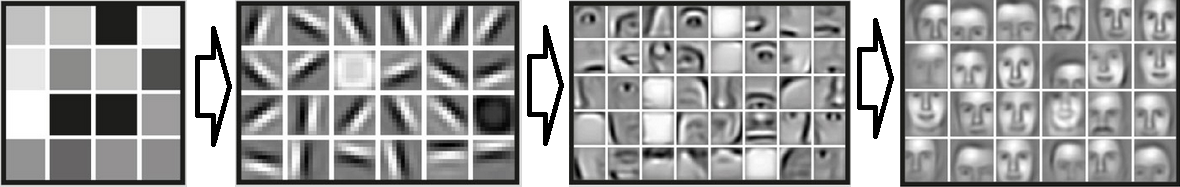
\includegraphics[width=0.95\linewidth]{images/1_Features}
\caption[Merkmale unterschiedlichen Abstraktionsgrads von links (Pixel) bis rechts (Gesichter)]{Merkmale unterschiedlichen Abstraktionsgrads von links (Pixel) bis rechts (Gesichter) (Einzelbilder: Andrew Ng, Stanford Artificial Intelligence Lab)}
\label{fig:1_Features}
\end{figure}
Den Beginn des heutigen Deep Learning stellt die Arbeit von \cite{Hinton2006} dar: Ein unüberwachtes Lernverfahren, welches tiefe Architekturen schichtweise mittels eines \textit{Greedy}-Algorithmus trainiert. Dadurch können, wie in Abbildung \ref{fig:1_Features} dargestellt, unterschiedliche Schichten Merkmale mit unterschiedlichem Abstraktionsgrad extrahieren. Die Gesamtstrategie sieht dabei vor, zuerst Merkmale unüberwacht zu extrahieren und diese im Anschluss für ein etwaiges überwachtes Lernverfahren, wie beispielsweise Kern-basierte Verfahren \cite[vgl.][]{Salakhutdinov2008}, zu verwenden. Dies ähnelt stark den Ideen von \cite{Becker1991}, die Principle Component Analysis (PCA) zur Vorverarbeitung der Trainingsdaten zu verwenden. Durch die tiefe, schichtweise Extraktion der Merkmale sind diese jedoch nicht exklusiv, sondern verteilt, was auch als \textit{Distributed Representation} bezeichnet wird \cite[vgl.][]{Hinton1986}.

In den vergangenen Jahren konnten so bahnbrechende Fortschritte im Bereich der Spracherkennung \cite[vgl][]{Sainatha2015}, der Verarbeitung natürlicher Sprache (NLP) \cite[vgl.][]{Socher2011} sowie  der Bilderkennung erzielt werden. Den aktueller Benchmark in Letzterem stellt das \textit{GoogLeNet} von \cite{Szegedy14} mit $26\%$ Top-5 Fehlern auf dem bekannten ImageNet-Problem\footnote{Der ImageNet-Datensatz besteht aus 200 Klassen, rund 450.000 Trainingsbeispielen, rund 20000 Beispielen zur Validierung und rund 40.000 Testbeispielen. Jedes Bild hat eine Größe von $482 \times 415 $  (\url{http://www.image-net.org/} (26.08.2015)).} \cite[vgl.][]{ImageNet2015}. Von den neuen Möglichkeiten im \textit{Deep Learning} profitieren auch die im letzten Kapitel erwähnten \textit{Convolutional Neural Networks} insofern, dass bestehende Ideen weiterentwickelt oder fehlende gelabelte Trainingsdaten kompensiert werden \cite[vgl.][]{LeRanzato2012}.\\

Heute werden unter \textit{Deep Learning} meist folgende fünf Modelle unterschieden:
\begin{itemize}
\item \textit{Recurrent Neural Network} (RNN) mit Long Short Term Memory (LSTM) (vgl. \cite{Hochreiter1997}
\item \textit{Convolutional Neural Network} (CNN)
	(vgl. \cite{LeCun1998}, \cite{Krizhevsky2012} und \cite{Simonyan2014})
\item \textit{Deep Belief Network} (DBNs) mit beschränkten Boltzmann-Maschinen (RBMs) 
	(vgl. \cite{Bengio2007} und \cite{Ranzato2007b})%Real valued
\item \textit{Stacked Denoising Autoencoder} (SDA) 
	(vgl. \cite{Vincent2008} und \cite{Vincent2010})
\item \textit{Deep Reinforcement Learning} (DRL) (vgl. \cite{Mnih2013})
\end{itemize}

\section{Ziel der Arbeit}
\label{ch:Ziele}
\textit{Convolutional Neural Networks} (CNNs) sind eine besondere Klasse von Neuronalen Netzen. Diese von der Neurobiologie inspirierten Modelle in Verbindung mit neueren Methoden aus dem Bereich \textit{Deep Learning}, stellen derzeit die besten Systeme für viele Probleme aus Bilderkennung, Spracherkennung und Verarbeitung natürlicher Sprache. 
Grundsätzlich werden drei Typen klassischer neuronaler Netze unterschieden: \textit{Single-Layer Feedforward Networks}, \textit{Multilayer Feedforward Networks} und \textit{Recurrent Networks} \cite[vgl.][S. 22f]{Haykin1999}, wobei rekurrente Varianten in dieser Arbeit nicht weiter betrachtet werden.

Diese Arbeit beschränkt sich auf \textit{Feedforward Networks} in den Bereichen Klassifikation und Regression und beschreibt somit das klassische, überwachte, neuronale Lernmodell.
Für den Entwurf dieser neuronalen Netze existieren bereits eine Vielzahl an Softwaretools. Als Beispiel werden hier folgende bekannten Softwareprodukte angeführt:
\begin{itemize}
\item Theano (Python) \cite[vgl.][]{Bergstra2010}

\item Torch (Lua) \cite[vgl.][]{Torch2011}

\item Cuda-Convnet (Cuda) \cite[vgl.][]{Nouri2013}

\item PyLean2 (Python) \cite[vgl.][]{PyLearn22013}

\item Caffe (C/C++) \cite[vgl.][]{Caffe2014}
\end{itemize}

Ziel dieser Arbeit ist es zum einen die Methoden im Bereich \textit{Deep Learning} aufzubereiten und zu analysieren. Darauf aufbauend wird ein eigener funktionierender Prototyp eines \textit{Convolutional Neural Networks} entwickelt. Dieser soll möglichst effizient sein, wenige Abhängigkeiten haben sowie eine Python-Schnittstelle bereitstellen. Im Zentrum der Untersuchungen stehen dabei überwachte Lernverfahren mit dem Ziel, Bilddaten mit \textit{State of the Art}-Performance zu klassifizieren, was allgemein als Bilderkennung bezeichnet wird. Darüber hinaus werden Methoden zum unüberwachten Vortraining und zur Visualisierung neuronaler Netze untersucht und vorgestellt.


Diese Arbeit entsteht am Institut für Optische Systeme (IOS) der HTWG Konstanz und dient zusammen mit zwei weiteren Arbeiten im Bereich \textit{Stacked Denoising Autoencoder} und \textit{LSTM-Recurrent Neural Network} als Grundlage für weitere Aktivitäten im Bereich \textit{Deep Learning} im IOS.


\section{Kapitelübersicht}
Diese Thesis ist unterteilt in sechs Kapitel. Kapitel 1 beginnt mit der thematischen Einordnung dieser Arbeit sowie der Motivation. Der Hauptteil ist in zwei Blöcke unterteilt. In Kapitel 2 und 3 werden notwendige Grundlagen für die Implementierung des Prototyps vorgestellt. So führt Kapitel 2 die Methode Neuronale Netze ausgehend vom Perzeptron ein und beschreibt im Speziellen die Besonderheiten der \textit{Convolutional Neural Networks} (CNNs). In Kapitel 3 werden spezielle Methoden des \textit{Deep Learning} vorgestellt. Der zweite Block besteht aus Kapitel 4 und 5. Kapitel 4 beschreibt die Entwicklung des Prototyps und Kapitel 5 die verschiedenen durchgeführten Experimente mit dem Ziel den Prototyp auf Richtigkeit zu überprüfen sowie verschiedene Aspekte im Deep Learning zu untersuchen. Im abschließenden 6. Kapitel werden die relevanten Ergebnisse der Arbeit nochmals zusammengefasst und ein Ausblick auf über diese Arbeit hinausgehende Aspekte gegeben.

